\documentclass[review]{elsarticle}

\usepackage{lineno,hyperref}
\usepackage{algorithm}
\usepackage{algorithmic}
\usepackage{amsmath,amssymb}
\usepackage{graphicx}
\usepackage{subfig}
\usepackage{tabularx}
\usepackage[usenames,dvipsnames]{xcolor}
\usepackage{colortbl}
\usepackage{amsmath}
\modulolinenumbers[5]

\journal{CIRP Journal of Manufacturing Science and Technology}

%%%%%%%%%%%%%%%%%%%%%%%
%% Elsevier bibliography styles
%%%%%%%%%%%%%%%%%%%%%%%
%% To change the style, put a % in front of the second line of the current style and
%% remove the % from the second line of the style you would like to use.
%%%%%%%%%%%%%%%%%%%%%%%

%% Numbered
%\bibliographystyle{model1-num-names}

%% Numbered without titles
%\bibliographystyle{model1a-num-names}

%% Harvard
%\bibliographystyle{model2-names.bst}\biboptions{authoryear}

%% Vancouver numbered
%\usepackage{numcompress}\bibliographystyle{model3-num-names}

%% Vancouver name/year
%\usepackage{numcompress}\bibliographystyle{model4-names}\biboptions{authoryear}

%% APA style
%\bibliographystyle{model5-names}\biboptions{authoryear}

%% AMA style
%\usepackage{numcompress}\bibliographystyle{model6-num-names}

%% `Elsevier LaTeX' style
\bibliographystyle{elsarticle-num}
%%%%%%%%%%%%%%%%%%%%%%%

\begin{document}

\begin{frontmatter}

\title{A Spatial AR System for Wide-area Axis-aligned Metric Augmentation of Planar Scenes} %\title{Elsevier \LaTeX\ template\tnoteref{mytitlenote}}
%\tnotetext[mytitlenote]{Fully documented templates are available in the elsarticle package on \href{http://www.ctan.org/tex-archive/macros/latex/contrib/elsarticle}{CTAN}.}

%% Group authors per affiliation:
\author{Michael Horn\'{a}\v{c}ek}\corref{mycorrespondingauthor}
\cortext[mycorrespondingauthor]{Corresponding author}
\ead{michael.hornacek@tuwien.ac.at}
\author{Hans K\"{u}ffner-McCauley}
\author{Majesa Trimmel}
\author{Patrick Rupprecht}
\author{Sebastian Schlund}
\address{Human Centered Cyber Physical Production and Assembly Systems, Institute for Management Sciences, TU Wien, Vienna, Austria}

\begin{abstract}
Augmented reality (AR) promises to enable use cases in industrial settings that include the embedding of assembly instructions directly into the scene, potentially reducing or altogether obviating the need for workers to refer to instructions in paper form or on a screen. \textit{Spatial} AR, in turn, is a form of AR whereby the augmentation of the scene is carried out using a projector, with the advantage of rendering the augmentation visible to all onlookers simultaneously without calling for each to wear some form of head-mounted display. Care must be taken in carrying out spatial AR, however, to warp the images to be projected in a manner that they appear free of distortions to the viewer, since the geometry of the scene as it relates to the geometry of the projector plays a role in how the pixels of the projector's image plane map to points in the scene. For planar scene geometry (such as a floor, wall, or table), this can be done in a cumbersome manual process called keystone correction, often using software bundled with the projector.

We propose a spatial AR system for wide-area metric augmentation of planar scene surfaces that produces the effect of keystone correction analytically, by using a projector equipped with a steerable mirror and a downwards-facing camera. Our system renders the placement of augmentations in the scene more intuitive than manual keystone correction in two ways. First, (i) placement of the desired augmentations is carried out in accordance with the axes of an image of the scene acquired by a camera placed to face downwards towards the scene plane; second, (ii) the desired dimensions of the projected augmentations is specified in metric terms. Our system produces such augmentations accurately, with compelling time savings relative manual keystone correction.
\end{abstract}

\begin{keyword}
Spatial augmented reality (SAR) \sep computer vision \sep projector calibration \sep Industry 4.0 \sep Pilotfabrik
\end{keyword}

\end{frontmatter}

\linenumbers

\section{Introduction}\label{sec:intro}

Augmented reality (AR) \cite{van2010survey,zhou2008trends} promises to enable use cases in industrial settings that include the embedding of assembly instructions directly into the scene \cite{schlund2018moglichkeiten,masood2019augmented,gattullo2019towards,rupprecht2020information,Rupprecht2021}, potentially reducing or altogether doing away with the need for workers to refer to instructions in paper form or on a screen. Typically, AR works by embedding the augmentation in an image of the scene acquired from the viewpoint of a single individual, with the resulting augmented image in turn displayed using some form of head-mounted display. Reliance on head-mounted displays, however, has two adverse consequences: (i) a head-mounted display must be worn by each individual wishing to partake in the augmentation, and (ii) such a head-mounted display---in some cases taking the form of a helmet in order to house multiple sensors in support of accurately tracking the viewpoint of the viewer relative to the scene---can be obtrusive. In turn, \textit{spatial} AR\cite{bimber2019spatial} is a form of augmented reality carried out not by embedding the augmentation in an image of the scene as with a head-mounted display, but by projection to the scene itself, thus eliminating both aforementioned problems. Yet considering a planar surface to be augmented (e.g., a floor, wall, or table), unless the projector faces the surface frontally, the bounds of a projected rectangular image will not appear rectangular, but will instead be subject to projective distortions. Such distortions can be eliminated by carrying out a cumbersome manual process called keystone correction to appropriately warp the image to be projected, often using software bundled with the projector.

Our contribution is to propose a wide-area spatial AR system for planar scenes that produces the effect of keystone correction analytically. Most importantly, we do this in a manner placing the axes of the augmentation in accordance with the axes of a camera placed to face downwards towards the scene plane. This facilitates placement of augmentations, since establishing the principal axes of the augmentation thus reduces to placing the downwards-facing camera in a manner such that the $X$- and $Y$-axes of the image align with the intended $X$- and $Y$-axes of the augmentation. We achieve this by warping the image to be projected using a plane-induced homography computed to produce the effect of projecting the image not from the actual projector viewpoint, but in accordance with the viewpoint of a \textit{virtual} projector (i) facing directly downwards to the target location in the scene plane and (ii) rotated to place the axes of the virtual projector in accordance with those of the camera. Moreover, our system enables specifying the dimensions of augmentations in metric terms, which we achieve by placing the virtual projector at the appropriate height above the scene plane. Finally, our system set up to handle a projector equipped with a steerable mirror (without need for explicitly modeling the action of the steerable mirror on the projector), thereby enabling wide-area factory floor applications exceeding the immediate field of view of the projector without needing to rely on multiple projectors.

\subsection{Related Work}

Keystone correction for planar scenes can be carried out using a 2D homography \cite{Hartley2004}---an invertible transformation that preserves colinearity, hence alternatively termed a `colineation'---and is ultimately the approach we take as well. The intuition for why it is that a transformation that maps lines to lines can serve to model the appropriate image warp can be drawn from considering a planar chessboard pattern: looking at an image of a chessboard acquired from an oblique angle, one observes that lines parallel in the chessboard appear to meet in respective vanishing points; looking at an image of the same chessboard acquired frontally with respect to the plane of the chessboard, lines parallel in the chessboard appear parallel in the image (i.e., they are said to meet `at infinity'). To warp the former image (where lines parallel in the scene meet in respective vanishing points) such that the lines of the chessboard appear as in the latter image (where lines parallel in the scene meet at infinity), a transformation that maps lines to lines would be sufficient.

One way to compute a homography is by identifying at least four correspondences between pixel positions in two images of a planar surface. The keystone correction approach of Sukthankar \textit{et al.} \cite{sukthankar2001smarter} reduces to using a segmentation approach to identify the four corners of projection screen in an image acquired by a camera, and computing a homography that maps the resulting four corners of the projection screen to the four corners of the projector's image plane. Tilt sensors can be used to recover the projector's gravity vector, and be integrated in the computation of a homography as in Raskar and Beardsley \cite{raskar2001self}.

An early spatial AR system explicitly using a projector with a steerable mirror is the IBM Everywhere Displays prototype of Pinhanez \cite{pinhanez2001everywhere}; the system, however, has keystone correction carried out manually. Rather than rely on a steerable mirror to support spatial AR to multiple locations using a single projector, some works mount the projector and a camera on a rigid rig and subject the rig to motion \cite{ehnes2004projected,borkowski2004spatial,butz2006applying}. Steering only a mirror, however, places humbler requirements on the system from a hardware standpoint than if an entire camera-projector rig is to be subject to rigid motion.

Mention asymmetrical circle pattern: \cite{chiu2011novel}


%todo: It consists of a projector and a small mirror with 2 axes of rotation. In contrast with the present work, Everywhere Displays is limited to projecting on a discrete set of planar surfaces which are calibrated beforehand, each modeled by a 2D homography. The Everywhere Displays project explored many applications of steerable displays, particularly in the retail domain. With the addition of a pan and tilt video camera, a number of gesture-based interactions are demonstrated, including touch-based manipulation of projected graphical widgets [12], as well as person tracking to enable graphics to follow the user. A small number of later works contribute steerable displays designs which mount the projector and camera directly onto motorized platform with pan and tilt axes of motion [8, 6, 11]. Butz et al. [7] contribute a number of interactions in the tradition of ubiquitous computing, such as the ability to 

\section{Approach}

Correcting for projective distortions of the sort outlined in Section~\ref{sec:intro} can be achieved by modeling the manner in which the respective rays through the pixels of the projector's image plane fan out into the scene (i.e., by `calibrating' the projector) and the geometry of the scene itself (i.e., by recovering the scene plane relative to the projector) within at least the projector's field of view. This is because the scene point `illuminated' by a pixel in the projector's image plane can be recovered by intersecting its corresponding ray with the geometry of the scene surface. To model this interaction, we (i) carry out a one-time projector calibration, which in our approach calls for additionally calibrating a camera facing downward to the scene plane and includes recovery of the scene plane as a convenient side effect. Next, we use the relative camera-projector-scene plane geometry to (ii) compute a plane-induced homography that warps the image to be projected in a manner that it appear undistorted to the viewer, and placed in alignment with the axes of a proxy image of the scene. These two points are treated in Sections~\ref{sec:approach:geometry} and \ref{sec:approach:homography}, respectively.

\subsection{Recovering Geometry}\label{sec:approach:geometry}

\begin{figure}
    \centering
    \subfloat[\centering Asymmetrical circle pattern image, in image plane of projector (detections overlain).]{{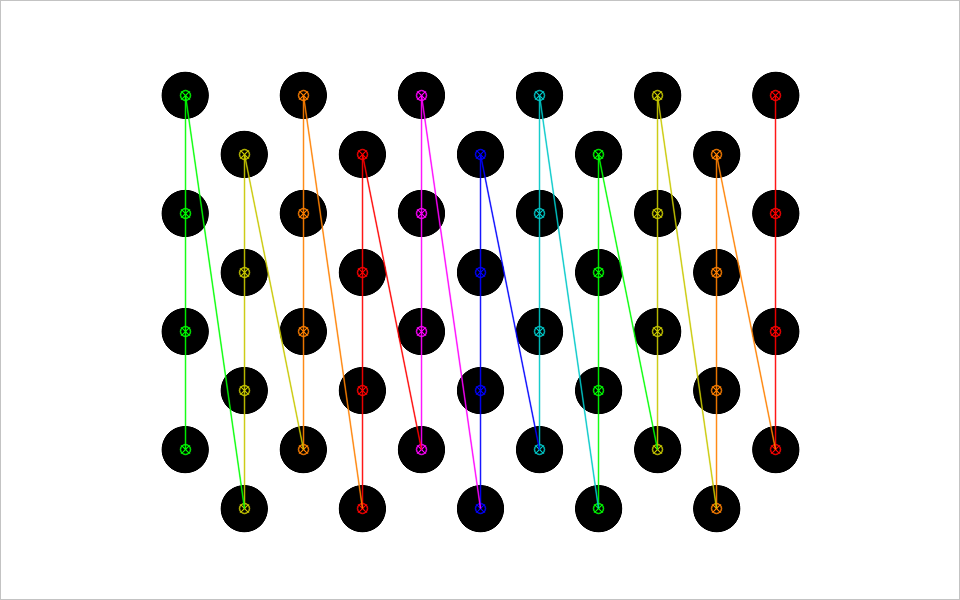
\includegraphics[height=3.25cm]{images/circles.png} }}
    \qquad
    \subfloat[\centering Projector calibration image (one for each target location), in image plane of camera (detections overlain).]{{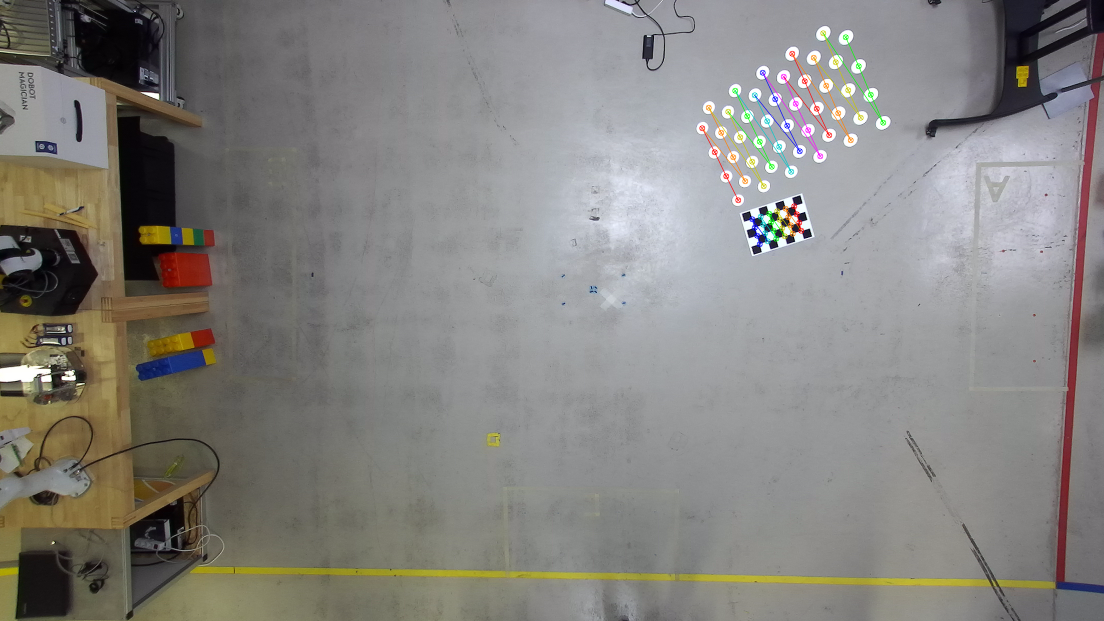
\includegraphics[height=3.25cm]{images/detections.png}}}
    \caption{Recovering 2D positions in support of projector calibration. (a) 2D positions of the 2D-3D correspondences to be used for calibrating the projector are obtained by detecting---in the image plane of the projector---the circle centers in the asymmetrical circle pattern image, to be projected to each of the target locations in the scene plane. (b) For each such target location, an image is acquired from the viewpoint of the camera and the circle centers of the projected asymmetrical circle pattern are detected, in the image plane of the camera. A chessboard pattern to be used for recovering the local scene plane is placed near the projected pattern, whose corners are likewise detected. Detected 2D projected asymmetrical circle pattern circle center points and chessboard corners overlain for illustration.}
    \label{fig:2d}
\end{figure}

Calibration of a projector (or camera) in the sense we employ the term here\footnote{We are referring to a geometric calibration; not, e.g., to a color calibration.} renders one able to project a scene point~$\mathbf{X} \in \mathbb{R}^3$ to its corresponding pixel~$\mathbf{x} \in \mathbb{R}^2$ in the projector's (or camera's) image plane, or to compute the `back-projection' of $\mathbf{x}$, i.e., the ray from the projector's (or camera's) center of projection through $\mathbf{x}$ along which a projecting point~$\mathbf{X}$ must lie. Such a calibration can be expressed in terms of (i) a $3~\times{}~3$ calibration matrix~$\mathtt{K}$ derived from the projector's (or camera's) focal length~$f$ and principal point~$\mathbf{p}_0 = (x_0, y_0)^\top \in \mathbb{R}^2$ \cite{Hartley2004}, and (ii)~the coefficients of a lens distortion model used to correct for radial or tangential distortions caused by the lens system \cite{duane1971close,weng1992camera}; the calibration matrix~$\mathtt{K}$ is then
\begin{equation}
\mathtt{K} = \begin{bmatrix}
f & 0 & x_0 \\
0 & f & y_0 \\
0 & 0 & 1
\end{bmatrix},
\end{equation}
where $f$ and $(p_x, p_y)^\top$ are both expressed in units of pixels.

Calibrating a camera can be carried out by relying on (i) establishing 2D-3D correspondences between pixels in the camera's image plane and the corresponding points in the scene, and on (ii) using those correspondences as input to an optimization procedure that relies on bundle adjustment \cite{triggs1999bundle} to output maximum likelihood estimates of the calibration matrix, the associated lens distortion model coefficients, and, for each calibration image, the pose (i.e., position and orientation) of the camera relative to the 3D points \cite{Hartley2004,zhang2000flexible}. Calibration images of a calibration surface such as a chessboard pattern are acquired from varying viewpoints using the camera, to be used to establish the 2D-3D correspondences~$\{\mathbf{x}_{i,j} \leftrightarrow \mathbf{X}_{i,j}\}$, $i \in \{ 1, \dots, n_\text{pt} \}, j \in \{ 1, \dots, n_\text{im} \}$, where $n_\text{pt}$ gives the number of correspondences obtained from one calibration image of the pattern, $n_\text{im}$ the number of such images, and $\mathbf{X}_{i,j} = \mathbf{X}_{i,j'}$, for $j, j' \in \{ 1, \dots, n_\text{im} \}$. Bundle adjustment is then used to obtain the maximum likelihood estimates~$(\hat{\omega}, \hat{\mathtt{K}}, \{(\hat{\mathtt{R}}_j, \hat{\mathbf{t}}_j)\})$ of the lens distortion model coefficients~$\omega$, calibration matrix~$\mathtt{K}$, and rigid body transformations $(\mathtt{R}_j, \mathbf{t}_j) \in SE(3)$ that minimize the cumulative reprojection error
\begin{equation}
%\sum_{i=0}^{n_\text{pt}} \sum_{j=0}^{n_\text{im}} d_\omega\big(\mathbf{x}_{i,j}, \pi_{\mathtt{K},\mathtt{R}_j,\mathbf{t}_j}(\mathbf{X}_{i,j})\big),
\sum_{i=1}^{n_\text{pt}} \sum_{j=1}^{n_\text{im}} d_{\hat{\omega}}(\mathbf{x}_{i,j}, \hat{\mathbf{x}}_{i,j}'),
\label{re}
\end{equation}
where $\hat{\mathtt{R}}_j\mathbf{X}_{i,j} + \hat{\mathbf{t}}_j \in \mathbb{R}^3$ expresses $\mathbf{X}_{i,j}$ in the camera coordinate frame of the camera corresponding to the $j^{\text{th}}$~calibration image and $(\hat{\mathbf{x}}_{i,j}'^\top, 1)^\top \sim \hat{\mathtt{K}}(\hat{\mathtt{R}}_j\mathbf{X}_{i,j} + \hat{\mathbf{t}}_j) \in \mathbb{P}^2$ gives the projection~$\hat{\mathbf{x}}_{i,j}' \in \mathbb{R}^2$ of the point~$\mathbf{X}_{i,j}$ to that image. The function~$d_{\hat{\omega}}$ is a distance function that computes a distance with respect to two pixel positions that it first corrects for lens distortions, in accordance with the lens distortion model coefficients~$\hat{\omega}$ \cite{duane1971close,weng1992camera}. The inverse rigid body transformation~$(\hat{\mathtt{R}}_j^{-1}, -\hat{\mathtt{R}}_j^{-1}\hat{\mathbf{t}}_j^{})$ gives the pose of the $j^{\text{th}}$~camera relative to the 3D points~$\{ \mathbf{X}_{i,j} \}$ of the calibration pattern.

Calibration of a projector can be carried out in precisely the same manner as calibrating a camera insofar as step (ii) is concerned; the major difference in projector calibration relative to the calibrating a camera concerns the manner in which 2D-3D correspondences are identified, i.e., between pixels in the image plane of the projector and the corresponding points in the scene. What remains of this section is concerned primarily with the recovery of 2D-3D correspondences in support of calibrating cameras and projectors. A consequence of the approach we take to identifying the 3D points of the 2D-3D correspondences we use for projector calibration is, for each target location, recovery of the pose of the scene plane relative to the coordinate frame of the camera.

\paragraph{Camera calibration} We recover 2D-3D correspondences in support of calibrating the downwards-facing camera by relying on a planar calibration surface to automatically identify correspondences between the 3D points on the calibration surface and their 2D correspondences in the image plane. The classical calibration surface is a chessboard pattern. The 3D corner points of the chessboard are obtained \textit{a priori} in a coordinate system defined in the plane of the chessboard\footnote{E.g., $(0,0,0), (1.5,0,0), (3,0,0), \dots, (9,7.5,0)$ for a chessboard with $7~\times{}~6$ corners ($8~\times{}~7$ squares), with each square of length and width of 1.5 unit, respectively. Note that the units of the chessboard's 3D points give the units in terms of which the camera calibration is carried out, and---owing to how our projector calibration relies on the camera calibration---the units of the projector calibration as well.}, requiring knowledge only of the dimensions of the chessboard pattern and of the length of a side of a chessboard square. The corresponding 2D points are obtained, in the same order, using a specialized algorithm \cite{bradski2000opencv}. A set of calibration images is acquired, each with the calibration pattern visible in a different part of the image plane, and such that the center and all corners and edges of the image plane are covered, the camera's autofocus setting be off, and the camera's zoom factor remain fixed. 2D-3D correspondences are then recovered for each calibration image, and the resulting list is passed on as input to an optimization procedure that relies on bundle adjustment to yield the camera calibration matrix~$\mathtt{K}_\text{cam}$. 

\paragraph{Projector calibration} As with camera calibration, projector calibration relies on 2D-3D correspondences, yet we obtain them in this case by \textit{projecting} a calibration pattern. The pattern we project is one of circles (cf.\ Figure~\ref{fig:2d}(a)), and we rely on an algorithm to detect the circle center points in the asymmetrical circle pattern in the image plane of the projector \cite{bradski2000opencv}, giving the 2D positions of our 2D-3D correspondences for calibrating the projector. We project the asymmetrical circle pattern to each of the target locations, and use the the calibrated downwards-facing camera to acquire a projector calibration image for each. Given a projector calibration image acquired using camera, we detect the circle centers of the \textit{projected} asymmetrical circle pattern (cf.\ Figure~\ref{fig:2d}(b)); given the scene plane (the recovery of which we shall return to in the paragraph that follows) and such a 2D circle center $\mathbf{x}$, we obtain its 3D correspondence by intersecting the back-projection~$\mathtt{K}_\text{cam}^{-1}(\mathbf{x}^\top, 1)^\top \in \mathbb{P}^2$ of $\mathbf{x}$ with the recovered scene plane (cf.\ Figure~\ref{fig:3d}). Since the algorithm that yields 2D circle centers does so in a consistent ordering, we thus obtain the 2D-3D correspondences between the projector's image plane and the scene required for projector calibration, yielding the projector calibration matrix~$\mathtt{K}_\text{proj}$.

\begin{figure}
    \centerline{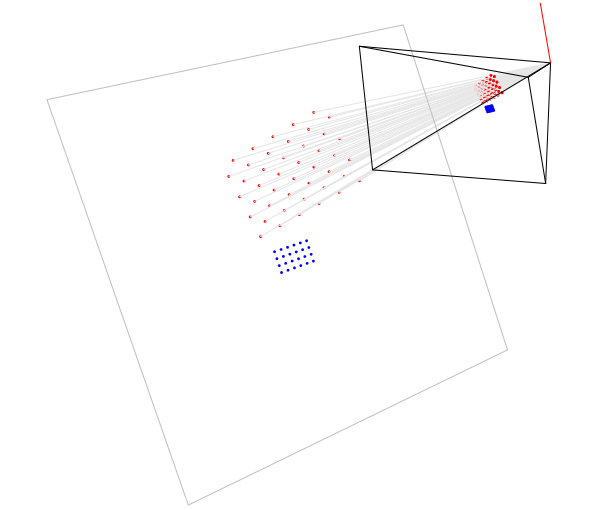
\includegraphics[scale=.35]{images/2d3d.png}}
    \caption{Scene plane (gray) recovered via spatial resection with respect to 2D-3D correspondences obtained using a chessboard pattern (blue); 3D circle center points of the asymmetrical circle pattern---i.e., the 3D positions of the 2D-3D correspondences to be used for calibrating the projector---obtained by intersection with the scene plane of back-projections (likewise gray) of the 2D circle center points of the asymmetrical circle pattern detected in the image plane (red). Note that as in the figures that follow, the rendering in the figure corresponds to the projection calibration image in Figure~\ref{fig:2d}(b), acquired by the downwards-facing camera (frustum of the camera in black, with up vector in red).}
    \label{fig:3d}
\end{figure}

We recover the scene plane via spatial resection by applying a PnP algorithm \cite{collins2014infinitesimal} to the 2D-3D correspondences obtained using a chessboard pattern. Note that this step is separate from camera calibration, yet could well be carried out using the same calibration pattern used in the camera calibration step.\footnote{The critical point is that the pattern should ideally be coplanar with the local scene plane, meaning its height above the scene plane should not exceed a few millimeters.} While a single image of such a chessboard pattern placed on the floor could be sufficient if the floor is even, we place a chessboard pattern in close proximity to the projected asymmetrical circle pattern in each projector calibration image in order to recover the scene plane locally to each target location, in order to account for the possibility of an uneven floor (cf.\ Figure~\ref{fig:2d}(b)). Note that in principle, we could project a chessboard pattern instead of an asymmetrical circle pattern to obtain the 2D-3D correspondences needed for projector calibration; it is, however, because we rely on detecting the corners of a chessboard pattern to recover the scene plane that we opt instead for a alternative pattern.

The pose of the projector, for each projector calibration image, is provided relative to the 3D points of the pattern---and thus in the coordinate frame of the camera---alongside $\mathtt{K}_\text{proj}$ by the aforementioned optimization procedure. Note that for a fixed projector with steerable mirror, given a projector calibration image, the recovered projector's pose is the pose the projector would have to have had to project to the given target location \textit{in the absence of the mirror}. This is sufficient for our needs in Section~\ref{sec:approach:homography}, and it is in this sense that our system is able to handle a projector equipped with a steerable mirror, without need for modeling the steerable mirror explicitly.

\begin{figure}
    \centering
    \subfloat[\centering Oblique view.]{{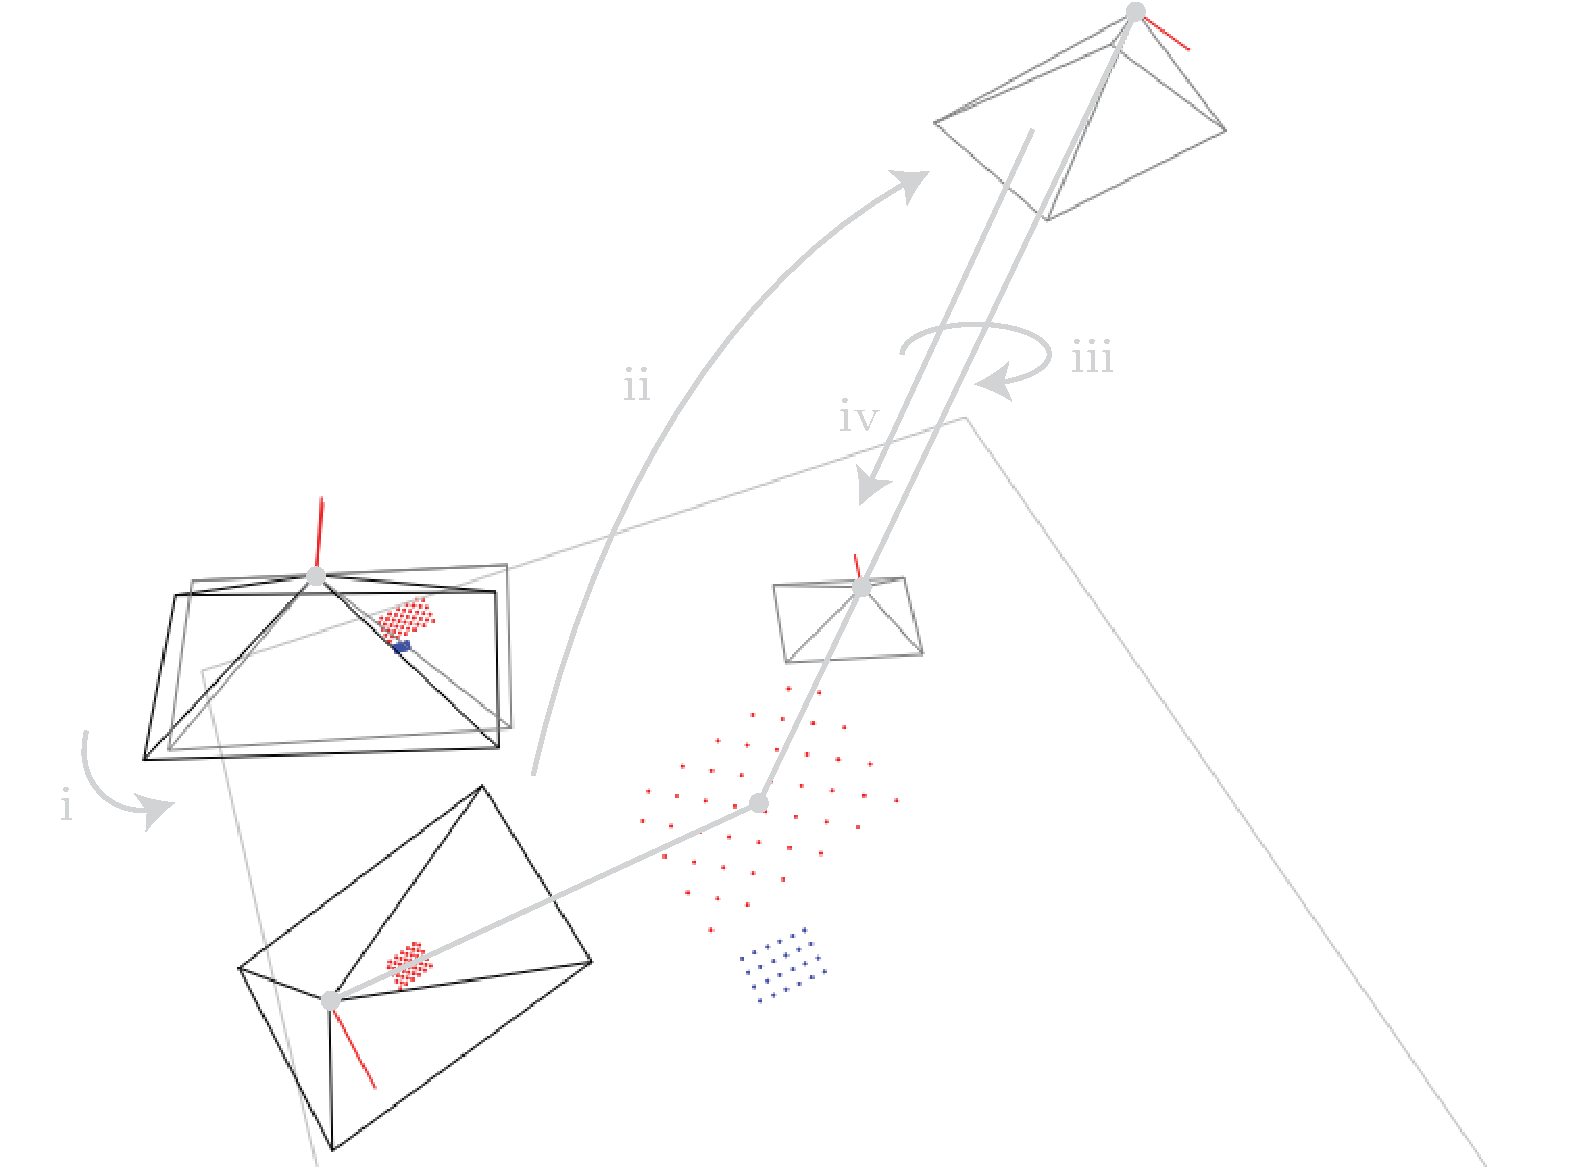
\includegraphics[height=4.2cm]{images/1.pdf}}}
    \qquad
    \subfloat[\centering Downwards view.]{{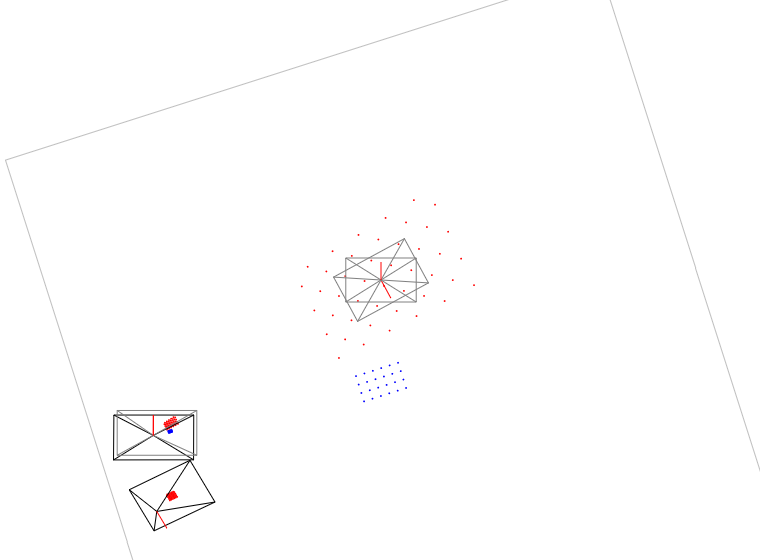
\includegraphics[height=4.2cm]{images/3_above3.png}}}
    \caption{The virtual camera is obtained by (i) rotating the camera (top left, black) about its center of projection such that its optical axis be made parallel with the normal vector of the scene plane. The virtual projector is obtained by (ii) rotating the projector (bottom left, black) about the point of intersection of its optical axis with the scene plane such that the optical axis be made parallel with the scene plane's normal vector, (iii) rotating the $X$- and $Y$-axes to align them with those of the virtual camera, and (iv) translating along the normal direction to achieve the desired metric projected image dimensions.} %The virtual projector is thus rendered fronto-parallel with the ground plane and axially aligned with the virtual camera.
    \label{fig:virtualproj}
\end{figure}

\subsection{Correcting for Projective Distortion}\label{sec:approach:homography}

If the projector is calibrated and its pose relative to the scene plane is known, a `virtual' projector (with the same calibration $\mathtt{K}$ and lens distortion model coefficients) can be placed elsewhere relative to the scene plane. If we for a moment imagine that the projector---at its recovered pose---functions as a camera,\footnote{Recall that the calibration matrix~$\mathtt{K}$ enables computing both (i) the projection of a scene point to the image plane (the function of a camera), or (ii) the back-projection of a pixel in the image plane, giving a ray into the scene (along which a projector illuminates the scene with the given pixel).} then (i) projecting an image to the scene plane \textit{from the viewpoint of the virtual projector} and (ii) acquiring the resulting projected image from the viewpoint of the recovered projector gives the desired corrective warp. Projecting an image warped in this manner to the scene plane \textit{from the viewpoint of the recovered projector} then has the same effect as projecting the original image to the scene plane from the viewpoint of the virtual projector. This warp can be effected using a plane-induced homography, computed analytically as a function of the scene plane, the projector, and the virtual projector.

\paragraph{Virtual projector} The placement of the virtual projector is to determine from which pose the image to be projected is to \textit{appear} to have been projected. We carry out this placement according to a small handful of steps. First, we (i) rotate the camera about its center of projection to align its optical axis\footnote{Strictly speaking, the optical axis is the back-projection of the principal point; in our usage, we understand it to refer to the back-projection of the center of the image to be projected.} with the normal vector of the scene plane, giving a virtual camera likewise facing directly\footnote{A physical camera placed to face downwards is almost certain to not face downwards precisely; in contrast, the virtual camera's optical axis is aligned exactly with the scene plane's normal vector, rendering it fronto-parallel with respect to the scene plane.} downwards to the scene plane (cf.\ Figure~\ref{fig:virtualproj}). Next, we (ii) intersect the scene plane with the optical axis (i.e., the ray from the projector's center of projection through the center of the image plane) and rotate the projector's placement about that point of intersection, aligning the optical axis with the scene plane's normal vector and giving an initial virtual projector. Finally, we (iii) align the $X$- and $Y$-axes of the initial virtual projector with those of the virtual camera, which gives the virtual projector (cf.\ again Figure~\ref{fig:virtualproj}). The virtual projector is thus rendered fronto-parallel with the scene plane, enabling projection to the scene plane absent of projective distortions. We additionally (iv) adjust the height above the scene plane of the virtual projector, in order to satisfy desired projected image dimensions provided in metric units.

Owing to the manner in which we place the virtual projector, the virtual projector's axes and thus the augmentation are aligned with the axes of the downward-facing camera; the placement of the camera thereby intuitively determines the principal axes according to which augmentations are to be placed. Note further that a consequence of placing the virtual projector by rotating about the point of intersection of the projector's optical axis with the scene plane is that \textit{the center of the projector's image plane remains invariant} to the placement of the virtual projector, i.e., a steerable mirror can be aimed with respect to a point projected from the center of the projector's image plane, further facilitating placement of augmentations.

\begin{figure}
    \centering
    \subfloat[\centering Projecting original image.]{{
\includegraphics[height=4.2cm]{images/proj_projim.png}}}
    \qquad
    \subfloat[\centering Projecting our warped image.]{{
\includegraphics[height=4.2cm]{images/proj_projim_waped.png}}}
    \caption{Projection to the scene plane from the recovered projector viewpoint (bottom left, black; virtual projector in center, gray) of the original image and of the warped image. (a) Projecting the original image to the scene plane. (b) After warping the original image according to our plane-induced homography for the given target location, the image is projected in a manner that appears free of projective distortions, aligned with the axes of the virtual camera (via the virtual projector), and to have the desired dimensions in the scene plane, expressed in metric units. Note that unprojected background is shown set to black.}
    \label{fig:warp}
\end{figure}

\paragraph{Plane-induced homography} Let $\mathtt{K}_\text{proj}$ express the calibration matrix of the recovered projector and $(\mathtt{R}, \mathbf{t}) \in SE(3)$ the rigid body transformation that transforms points from the coordinate frame of the recovered projector to that of the virtual projector, for a given target location. Moreover, let $(\mathbf{n}^\top, -d)^\top$ give the scene plane, expressed in the coordinate frame of the recovered projector, where $\mathbf{n} \in \mathbb{R}^3$ is the scene plane's normal vector and $d = \mathbf{n}^\top\mathbf{X}$ for any point~$\mathbf{X}$ in the plane, so that $(\mathbf{n}^\top, -d) (\mathbf{X}^\top, 1)^\top = 0$. The transformation that warps the image to be projected to the scene plane by the recovered projector such that it appear as if were projected to the scene plane by the virtual projector (cf.\ Figure~\ref{fig:warp}(b)) is given the by the $3~\times~3$ matrix
\begin{equation}
\mathtt{H} = \mathtt{K}_\text{proj}\left(\mathtt{R} - \frac{\mathbf{t}\mathbf{n}^\top}{d}\right)\mathtt{K}_\text{proj}^{-1},
\label{homgen}
\end{equation}
a form of `plane-induced' homography \cite{Hartley2004}. For convenience, we enable optional rotation of the image to be projected \textit{before} applying $\mathtt{H}$, about the image center; that rotation, parameterized in degrees, is thus in effect likewise carried out intuitively relative to the placement of the camera.

\section{Evaluation}

We evaluate our approach by augmenting 15 locations across the floorspace at the Pilotfabrik\footnote{\url{https://www.pilotfabrik.at/}} of TU Wien, a collaborative space for research on Industry 4.0 topics situated in Vienna, Austria. We contrast our approach with a baseline approach involving manual keystone correction, by aiming with both approaches to place the same image for each location aligned with the principal axes of the floorspace, absent of projective distortions, and with the same metric dimensions (50~cm~$\times$~31.25~cm\footnote{The dimensions in pixels of the image we project are 960~$\times$~600; we chose for our experiments to set the projected metric length of the horizontal axis of the image to 50~cm, which implies 31.25~cm for the vertical axis if aspect ratio is to be preserved.}). All experiments were carried out by the same technician, experienced in both approaches.

The hardware setup employed in the evaluation comprised a Panasonic PT-RZ660BE projector with a steerable mirror system---used in our experiments to point the projection to each of the 15 locations---manufactured by Dynamic Projection Institute \cite{rupprecht2020information,Rupprecht2021}. The steerable mirror system was bundled with the MDC-X software for steering the mirror, loading imagery, and optionally carrying out manual keystone correction, such that each position and (warped) image can be registered as a preset. In addition, we used a downward-facing Zed 2 stereo camera manufactured by Stereolabs, yet relied only on the left view. The floorspace used for our experiments measured dimensions of ca.\ 6~m~$\times$~4~m; the projector was mounted at approximately the center of this space, at a height of ca.\ 3.5 m.

\paragraph{Manual approach} ...

\paragraph{Our approach} We began by carrying out a calibration of the camera, acquiring 10 camera calibration images (cf.\ Section~\ref{sec:approach:geometry}) of a chessboard calibration pattern with $6~\times~4$ corners ($7~\times~5$ squares) and feeding the images as input to our camera calibration module. Separately, for each of the 15 target locations, we produced a projector calibration image (cf.\ again Section~\ref{sec:approach:geometry}) by projecting a $11~\times~4$ asymmetrical circle pattern image to the location in question using the steerable mirror, placing a checkerboard pattern beside the projected pattern, and acquiring the image using the downward-facing camera. We then fed these images alongside the output of the camera calibration module to our projector calibration module. For each of the target locations, the steerable mirror was made to point to that location, the asymmetrical circle pattern image was projected to the scene plane, an image was using the camera, and the location was registered in the MDC-X software as a preset. The output of the projector calibration module is a homography per input projector calibration image (cf.\ Section~\ref{sec:approach:homography}). Next, we warped the images to be projected to the respective locations using their corresponding homography, using a third dedicated custom module. These warped images were finally imported into the MDC-X software and associated with their respective location presets.

The total amount of time to carry out all the above steps amounted to ca.\ 20 min, with ca.\ 2 min going to acquisition of the camera calibration images, and ca.\ 5 min going to that of projector calibration images. The remainder of the time was spent running our modules or working with the MDC-X software. Note that once the camera is calibrated, that calibration can be reused if the camera's intrinsics remain fixed, in particular if no change is made to the zoom factor of the camera.

\section{Conclusion}

We presented a spatial AR system for planar scenes that produces the effect of keystone correction analytically, in a manner that enables intuitive placement the augmentations in accordance with the axes of an image of the scene acquired by a downwards-facing camera, and such that the desired dimensions of augmentations can be specified in metric terms. Moreover, we showed our system to be able to handle a projector equipped with a steerable mirror, enabling factory floor augmentation exceeding the bounds of the projector's own immediate field of view. Our evaluation demonstrated our approach to produce compelling results at less time than the more cumbersome traditional manual approach to keystone correction.

A natural extension of this work would be to address non-planar scenes. To handle non-planar scenes would call for a change in how scene geometry is recovered and how warping of the image to be projected is carried out; the methodology we proposed for projector calibration could, however, be left unchanged.

\section{Acknowledgments}

This work was supported by the Austrian Research Promotion Agency (FFG) through its endowed professorship in Human Centered Cyber Physical Production and Assembly Systems at TU Wien (FFG-852789).

\bibliography{mybibfile}

\end{document}

% idea for next work: LM-based approach to globally recover scene plane from projected patterns (try to make a patent of this!)... compute intersection of optical axes of all recovered projectors - it is about this point that the projector can be steered in terms of angles; once scene plane is availabe, intrinsics of projector are available, and the 'steering point' is available, we can have a GUI with which you click on an undistorted image of the scene plane to control the steerable mirror
